%!TEX TS-program = xelatex
%!TEX encoding = UTF-8 Unicode
% Awesome CV LaTeX Template for CV/Resume
%
% This template has been downloaded from:
% https://github.com/posquit0/Awesome-CV
%
% Author:
% Claud D. Park <posquit0.bj@gmail.com>
% http://www.posquit0.com
%
% Template license:
% CC BY-SA 4.0 (https://creativecommons.org/licenses/by-sa/4.0/)
%


%-------------------------------------------------------------------------------
% CONFIGURATIONS
%-------------------------------------------------------------------------------
% A4 paper size by default, use 'letterpaper' for US letter
\documentclass[11pt, a4paper]{awesome-cv}
\usepackage[T1]{fontenc}
\usepackage[utf8]{inputenc}

% Configure page margins with geometry
\geometry{left=1.4cm, top=.8cm, right=1.4cm, bottom=1.8cm, footskip=.5cm}

% Color for highlights
% Awesome Colors: awesome-emerald, awesome-skyblue, awesome-red, awesome-pink, awesome-orange
%                 awesome-nephritis, awesome-concrete, awesome-darknight
\colorlet{awesome}{awesome-red}
% Uncomment if you would like to specify your own color
% \definecolor{awesome}{HTML}{CA63A8}

% Colors for text
% Uncomment if you would like to specify your own color
% \definecolor{darktext}{HTML}{414141}
% \definecolor{text}{HTML}{333333}
% \definecolor{graytext}{HTML}{5D5D5D}
% \definecolor{lighttext}{HTML}{999999}
% \definecolor{sectiondivider}{HTML}{5D5D5D}

% Set false if you don't want to highlight section with awesome color
\setbool{acvSectionColorHighlight}{true}

% If you would like to change the social information separator from a pipe (|) to something else
\renewcommand{\acvHeaderSocialSep}{\quad\textbar\quad}
\newcommand{\githublogo}{\faGithub}
\newcommand{\gitlogo}{
\includegraphics[height=0.25cm]{logos/git.png}}
\newcommand{\cpplogo}{
\includegraphics[height=0.25cm]{logos/C++.png}}
\newcommand{\clogo}{
\includegraphics[height=0.25cm]{logos/C.png}}
\newcommand{\pythonlogo}{
\includegraphics[height=0.25cm]{logos/Python.png}}
\newcommand{\numpylogo}{
\includegraphics[height=0.25cm]{logos/numpy.png}}
\newcommand{\scipylogo}{
\includegraphics[height=0.25cm]{logos/scipy.png}}
\newcommand{\matplotliblogo}{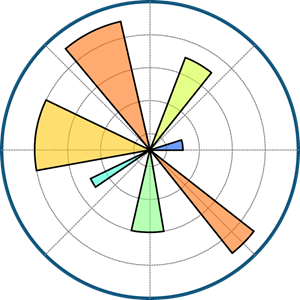
\includegraphics[height=0.25cm]{logos/matplotlib.png}}
\newcommand{\keraslogo}{
\includegraphics[height=0.25cm]{logos/keras.png}}
\newcommand{\mathematicalogo}{
\includegraphics[height=0.25cm]{logos/Mathematica.png}}
\newcommand{\tensorflowlogo}{
\includegraphics[height=0.25cm]{logos/tensoflow.png}}
\newcommand{\linuxlogo}{
\includegraphics[height=0.25cm]{logos/linux.png}}
\newcommand{\gnulogo}{
\includegraphics[height=0.25cm]{logos/gnu.png}}
\newcommand{\latexlogo}{
\includegraphics[height=0.25cm]{logos/LaTeX.png}}
\newcommand{\bashlogo}{
\includegraphics[height=0.25cm]{logos/bash.png}}
\newcommand{\fortranlogo}{
\includegraphics[height=0.25cm]{logos/Fortran.png}}
\newcommand{\vscodelogo}{
\includegraphics[height=0.25cm]{logos/vscode.png}}
\newcommand{\vimlogo}{
\includegraphics[height=0.25cm]{logos/Vim.png}}
\newcommand{\emacslogo}{
\includegraphics[height=0.25cm]{logos/emacs.png}}
\newcommand{\cmakelogo}{
\includegraphics[height=0.25cm]{logos/Cmake.png}}
\newcommand{\sqlitelogo}{
\includegraphics[height=0.25cm]{logos/Sqlite.png}}
\newcommand{\numbalogo}{
\includegraphics[height=0.25cm]{logos/Numba.png}}
\newcommand{\slurmlogo}{
\includegraphics[height=0.25cm]{logos/slurm.png}}
\newcommand{\pbslogo}{
\includegraphics[height=0.25cm]{logos/pbs.png}}
% \newcommand{\githublogo}{\textcolor{teal}{\textbf{github}}}
% \newcommand{\inspire}{\aiicon{inspire}}
\newcommand{\inspire}{\textcolor{awesome-red}{\textbf{Inspire}}}
\newcommand{\adalogo}{
\includegraphics[height=0.25cm]{logos/ada_logo2.png}}
\newcommand{\doorslogo}{
\includegraphics[height=0.25cm]{logos/doors_logo.png}}
\newcommand{\rtclogo}{
\includegraphics[height=0.25cm]{logos/rtc_logo.png}}
\newcommand{\windowslogo}{
\includegraphics[height=0.25cm]{logos/windows_logo.png}}
\newcommand{\officelogo}{
\includegraphics[height=0.25cm]{logos/microsoftoffice_logo.png}}
\newcommand{\qtlogo}{
\includegraphics[height=0.25cm]{logos/qt.png}}
\newcommand{\gnatlogo}{
\includegraphics[height=0.25cm]{logos/gnatstudio_logo.png}}
\newcommand{\wiresharklogo}{
\includegraphics[height=0.25cm]{logos/wireshark_logo.png}}
\newcommand{\xmllogo}{
\includegraphics[height=0.25cm]{logos/xml_logo.png}}

\usepackage{academicons}
\usepackage{fontawesome5}
\usepackage{tcolorbox}
\usepackage{xcolor}

%-------------------------------------------------------------------------------
%	PERSONAL INFORMATION
%	Comment any of the lines below if they are not required
%-------------------------------------------------------------------------------
% Available options: circle|rectangle,edge/noedge,left/right
% \photo{./examples/profile.png}
\name{Niccol\`o}{Laurenti}
% \name{Prova}{Prova}
\position{Ph.D.\ Graduate in Particle Physics~~~·~~~Software Developer}
% \position{Site Reliability Engineer{\enskip\cdotp\enskip}Software Architect}
% \address{via Leonida Rech 80, Rome, 00156, Italy}

\mobile{(+39) 3382971956}
\email{niclaurenti@gmail.com}
% \dateofbirth{March 17th, 1997}
\linkedin{niccolo-laurenti}
\github{niclaurenti}
\homepage{https://niclaurenti.github.io}
\orcid{0009-0001-0718-0409}

% \gitlab{gitlab-id}
% \stackoverflow{SO-id}{SO-name}
% \twitter{@twit}
% \skype{skype-id}
% \reddit{reddit-id}
% \medium{medium-id}
% \kaggle{kaggle-id}
% \hackerrank{hackerrank-id}
% \googlescholar{googlescholar-id}{name-to-display}
%% \firstname and \lastname will be used
% \googlescholar{googlescholar-id}{}
% \extrainfo{extra information}

% \quote{``Be the change that you want to see in the world."}


%-------------------------------------------------------------------------------
\begin{document}

% Print the header with above personal information
% Give optional argument to change alignment(C: center, L: left, R: right)
\makecvheader

% Print the footer with 3 arguments(<left>, <center>, <right>)
% Leave any of these blank if they are not needed
\makecvfooter
  {\today}
  {Niccol\`o Laurenti~~~·~~~Curriculum Vitae}
  {\thepage}


%-------------------------------------------------------------------------------
%	CV/RESUME CONTENT
%	Each section is imported separately, open each file in turn to modify content
%-------------------------------------------------------------------------------

% %-------------------------------------------------------------------------------
%	SECTION TITLE
%-------------------------------------------------------------------------------
\cvsection{Summary}


%-------------------------------------------------------------------------------
%	CONTENT
%-------------------------------------------------------------------------------
\begin{cvparagraph}

%---------------------------------------------------------
Ph.D.\ graduate in theoretical particle physics specialised in applying artificial intelligence to investigate
proton structure.
I am currently working as embedded software developer in the defence sector.
I have experience working with different programming languages, in particular with \texttt{C++} and \texttt{Python}.
I have hands-on experience with various machine learning tools like \texttt{Keras} and \texttt{Tensorflow}.
%Passionate about the field of computer science and eager to learn new things to further improve my skills.
\end{cvparagraph}
%-------------------------------------------------------------------------------
%	SECTION TITLE
%-------------------------------------------------------------------------------
\cvsection{Personal Informations}


%-------------------------------------------------------------------------------
%	CONTENT
%-------------------------------------------------------------------------------
\begin{cvskills}

    %---------------------------------------------------------
    \cvskill
        {Birth} % Category
        {1997, Rome, Italy} % Skills

    %---------------------------------------------------------
    % \cvskill
    %     {Place of birth} % Category
    %     {Rome, Italy} % Skills

    %---------------------------------------------------------
    \cvskill
        {Citizenship} % Category
        {Italian} % Skills
    
    %---------------------------------------------------------
    \cvskill
        {Languages} % Category
        {Italian (native language), English (fluent)} % Skills

    %---------------------------------------------------------
\end{cvskills}
\cvsection{Experience}


%-------------------------------------------------------------------------------
%	CONTENT
%-------------------------------------------------------------------------------
\begin{cventries}

%---------------------------------------------------------
  \cventry
  {Researcher in Theoretical Particle Physics at the University of Milan and INFN}
  {Ph.D.\ Researcher}
  {Milan, Italy}
  {Oct.\ 2021 - current}
  {
      \begin{cvitems} % Description(s) of tasks/responsibilities
        \item During my Ph.D., I worked under the supervision of Prof.\ Stefano Forte in the \href{https://nnpdf.mi.infn.it}{NNPDF collaboration} as a developer of the \href{https://github.com/NNPDF}{NNPDF code}.
        My role involved developing techniques and computational programs applied to particle physics.
        The aim of the research project was to utilize artificial intelligence to investigate, with high precision,
        the internal structure of the proton analyzing experimental data collected at \href{https://home.cern}{CERN}.
        \item The results of the work have been published in three papers and have been presented in conferences.
        \item Furthermore, during this period, I worked as a Teaching Assistant and Lecturer for both Bachelor's and Master's courses. 
      \end{cvitems}
    }

    \cventry
{Researcher in Theoretical Particle Physics at the University of Rome ``La Sapienza''}
{Undergraduate Researcher}
{Rome, Italy}
{Mar.\ 2021 - Oct.\ 2021}
{
      \begin{cvitems} % Description(s) of tasks/responsibilities
        \item During my Master Thesis I worked, under the supervision of Dr.\ Marco Bonvini and in collaboration with another Master student,
        to develop theoretical methods and computational programs to produce high-precision theoretical predictions in particle physics.
        These predictions aimed to describe experimental data collected at the particle accelerator \href{https://en.wikipedia.org/wiki/HERA_(particle_accelerator)}{HERA}.
        \item As a result of the work, two programs have been written, \href{https://github.com/niclaurenti/adani}{\texttt{Adani}} and \href{https://github.com/andreab1997/DIS_TP}{\texttt{DIS\_TP}},
        a paper has been published and the results have been presented in conferences.
      \end{cvitems}
    }


\end{cventries}
%-------------------------------------------------------------------------------
%	SECTION TITLE
%-------------------------------------------------------------------------------
\cvsection{Skills}


%-------------------------------------------------------------------------------
%	CONTENT
%-------------------------------------------------------------------------------
\begin{cvskills}

    %---------------------------------------------------------
    \cvskill
        {Programming} % Category
        {C, C++, Python, Fortran, Bash, Git, VS Code, Docker} % Skills

    %---------------------------------------------------------
    \cvskill
        {Operating systems} % Category
        {Linux, MacOS, Windows} % Skills

    %---------------------------------------------------------
    \cvskill
        {Scientific packages} % Category
        {GSL, Numpy, Scipy, Matplotlib, Pandas, Keras, Tensorflow, SQLite} % Skills

    %---------------------------------------------------------
    \cvskill
        {Scientific programs} % Category
        {Matlab, Mathematica} % Skills

    %---------------------------------------------------------

    %---------------------------------------------------------
    \cvskill
        {Writing} % Category
        {Latex, Markdown, Microsoft Office} % Skills

    %---------------------------------------------------------
\end{cvskills}
%-------------------------------------------------------------------------------
%	SECTION TITLE
%-------------------------------------------------------------------------------
\cvsection{Education}


%-------------------------------------------------------------------------------
%	CONTENT
%-------------------------------------------------------------------------------
\begin{cventries}

    %---------------------------------------------------------
    \cventry
        {University of Milan} % Institution
        {Ph.D.\ in Physics} % Degree
        {Milan, Italy} % Location
        {Oct.\ 2021 - current} % Date(s)
        {
        \begin{cvitems} % Description(s) bullet points
            \item Field of study: Theoretical Particle Physics, Computational Physics.
            \item Graduating in fall 2024.
        \end{cvitems}
        }

    %---------------------------------------------------------
    \cventry
        {University of Rome ``La Sapienza''} % Institution
        {M.S.\ in Physics} % Degree
        {Rome, Italy} % Location
        {Sep.\ 2019 - Oct.\ 2021} % Date(s)
        {
        \begin{cvitems} % Description(s) bullet points
            \item Field of study: Theoretical Particle Physics.
            \item Grade: 110/110 (cum laude).
            \item Thesis: \href{https://arxiv.org/pdf/2401.12139.pdf}{\emph{Construction of a next-to-next-to-next-to-leading order approximation for heavy flavour production in deep inelastic scattering with quark masses}}.
        \end{cvitems}
        }

    %---------------------------------------------------------
    \cventry
        {University of Rome ``La Sapienza''} % Institution
        {B.S.\ in Physics} % Degree
        {Rome, Italy} % Location
        {Sep.\ 2016 - Nov.\ 2019} % Date(s)
        {
        \begin{cvitems} % Description(s) bullet points
            \item Grade: 110/110 (cum laude).
            \item Thesis: \emph{Particle identification with the time of flight method and applications to the CMS experiment}.
        \end{cvitems}
        }

    %---------------------------------------------------------
\end{cventries}
\cvsection{Publications}

\begin{cvhonors}

    %---------------------------------------------------------
    \cvhonor
    {Implementation of DIS at N$^3$LO for PDF determination} % Category
    {A.\ Barontini, M.\ Bonvini, N.\ Laurenti} % Skills
    {}
    {2024}
    
    \cvhonor
    {The Path to N$^3$LO Parton Distributions} % Category
    {The NNPDF Collaboration, R.\ D.\ Ball et al.} % Skills
    {}
    {2024}
    
    \cvhonor
    {\href{https://arxiv.org/pdf/2401.10319.pdf}{Determinantion of the theory uncertainties from missing higher orders on NNLO parton distributions with percent accuracy}} % Category
    {The NNPDF Collaboration, R.\ D.\ Ball et al., \emph{Eur.\ Phys.\ J.\ C}} % Skills
    {}
    {2024}
    
    \cvhonor
    {\href{https://arxiv.org/pdf/2401.08749.pdf}{Photons in the proton: implications for the LHC}} % Category
    {The NNPDF Collaboration, R.\ D.\ Ball et al., \emph{Eur.\ Phys.\ J.\ C}} % Skills
    {}
    {2024}

    \cvhonor
    {\href{https://doi.org/10.1016/j.nuclphysbps.2023.11.013}{Inclusion of QED corrections in PDFs fits}}
    {N.\ Laurenti, \textit{Nuclear and Particle Physics Proceedings}}
    {}
    {2023}
    
    \cvhonor
    {\href{https://arxiv.org/abs/2207.12265}{Approximating missing higher-orders in transverse momentum distributions using resummations}}
    {N.~Laurenti, T.\ R.\ Rabemananjara, and R.\ Stegeman}
    {}
    {2022}

    %---------------------------------------------------------
\end{cvhonors}
\cvsection{Talks}
\begin{cvhonors}

    %---------------------------------------------------------
    \cvhonor
    {Evidence of intrinsic charm quarks in the proton} % Category
    {Mainz, Germany}
    {\href{https://indico.him.uni-mainz.de/event/171/}{MENU23}} % Skills
    % {20 Oct. 2023}
    {2023}

    \cvhonor
    {Including QED corrections in PDF fits: The NNPDF4.0QED PDF set} % Category
    {Durham, UK}
    {\href{https://conference.ippp.dur.ac.uk/event/1128/}{QCD@LHC23}} % Skills
    % {5 Sept 2023}
    {2023}

    \cvhonor
    {Inclusion of QED corrections in PDFs: The NNPDF4.0QED PDF set} % Category
    {Montpellier, France}
    {\href{https://qcd23.sciencesconf.org/}{QCD23}} % Skills
    % {10 July 2023}
    {2023}

    \cvhonor
    {Construction of a third order approximation for heavy flavour production in deep inelastic scattering} % Category
    {Milan, Italy}
    {\href{https://indico.cern.ch/event/1095418/}{MCM 2021}} % Skills
    % {21 Dec 2021}
    {2021}
    
    


    %---------------------------------------------------------
\end{cvhonors}
\cvsection{Teaching activity}

\begin{cvhonors}

    %---------------------------------------------------------
    \cvhonor
    {TA for the course of Quantum Physics I} % Category
    {Introduction to Quantum Mechanics}
    {University of Milan} % Skills
    {2024}

    \cvhonor
    {TA for the course of Physics} % Category
    {Basics of Classical Mechanics and Thermodynamics}
    {University of Milan} % Skills
    {2024}

    \cvhonor
    {TA for the course of Quantum Physics II} % Category
    {Advanced course on Quantum Mechanics}
    {University of Milan} % Skills
    {2024}

    \cvhonor
    {TA for the course of Theoretical Physics I} % Category
    {Introduction to Quantum Field Theory}
    {University of Milan} % Skills
    {2023}

    \cvhonor
    {TA for the course of Physics} % Category
    {Basics of Classical Mechanics and Thermodynamics}
    {University of Milan} % Skills
    {2023}

    \cvhonor
    {TA for the course of Quantum Physics II} % Category
    {Advanced course on Quantum Mechanics}
    {University of Milan} % Skills
    {2023}

    \cvhonor
    {Exercise classes for the course of Quantum Physics II} % Category
    {Advanced course on Quantum Mechanics}
    {University of Milan} % Skills
    {2023}

    \cvhonor
    {TA for the course of Quantum Physics I} % Category
    {Introduction to Quantum Mechanics}
    {University of Milan} % Skills
    {2022}

    
    


    %---------------------------------------------------------
\end{cvhonors}
% %-------------------------------------------------------------------------------
%	SECTION TITLE
%-------------------------------------------------------------------------------
\cvsection{Others}


%-------------------------------------------------------------------------------
%	SUBSECTION TITLE
%-------------------------------------------------------------------------------
% \cvsubsection{International Awards}


%-------------------------------------------------------------------------------
%	CONTENT
%-------------------------------------------------------------------------------
\begin{cventries}

%---------------------------------------------------------
  \cventry
  {University of Rome ``La Sapienza'', SoRT} % Location
    {Student Collaboration Scholarship} % Event
    {Rome, Italy}
    {2021} % Date(s)
    {
      \begin{itemize} % Description(s) of tasks/responsibilities
        \item I won one of the 39 collaboration scholarships at the Physics department of the University of Rome 
        ``La Sapienza''.
        All informations can be gathered from the official page \url{https://www.uniroma1.it/en/pagina/student-collaboration-scholarships}.
      \end{itemize}
    }
%---------------------------------------------------------
\end{cventries}


%-------------------------------------------------------------------------------
\end{document}